\chapter{Contour integration and border-ownership assignment}
\label{sec:contour}
\chaptermark{Contour integration and border ownership}

\section{Introduction}
\label{intro}

Gestalt psychologists recognized the importance of the whole in
influencing perception of the parts when they laid out several
principles (``Gestalt laws'') for perceptual
organization~\citep{Wertheimer23,Koffka35}. Contour integration, the
linking of line segments into contours, and figure-ground segregation,
the segmenting of objects from background, are fundamental components
of this process. Both require combining local, low-level and global,
high-level information across different visual areas in order to
segment the visual scene. The interaction between feedforward and
feedback streams carrying this information, as well as the
contribution of top-down influences such as attention, are not well
understood. 

The contour integration process begins in primary visual cortex (V1),
where the responses of orientation selective neurons can be modulated
by placing collinear stimuli outside the receptive fields (RFs) of
these neurons~\citep{Stemmler_etal95a,Polat_etal98}. Contextual
interactions between V1 neurons have often been summarized using a
``local association field,'' where collinear contour elements excite
each other and noncollinear elements inhibit each other
\citep{Ullman92, Field_etal93}.  Results from neuroanatomy lend
support to these ideas, as the lateral connections within V1
predominantly link similar-orientation cortical columns
\citep{Gilbert_Wiesel89,Bosking_etal97,
  Stettler_etal02}. Computational models based on these types of local
interactions have successfully explained the ability of V1 neurons to
extract contours from complex
backgrounds~\citep{Li98,Yen_Finkel98,Piech_etal13}. While some of
these models incorporate a combination of feedback and lateral
connections, the mechanisms by which higher visual areas construct the
appropriate feedback signals and target early feature neurons are not
clearly specified.  
\comment{One of the main purposes of the present study is
to introduce concrete neural circuitry that makes this recurrent
structure explicit, thereby allowing us to make quantitative
predictions and compare model predictions with experimental data.}

Segmenting an image into regions corresponding to objects requires not only finding the contours in the image but also determining which contours belong to which objects.
% don't mention binding problem
\comment{This is part of what is known as the {\em binding problem,} as it is unclear how higher visual areas ``know'' which features belong to an object~\citep{Treisman96b}.
One solution involves differential
neural activity, where the neurons responding to the features of an
object show increased firing compared with neurons responding to the
background.  Such response enhancement was first observed in V1 for texture-defined
figures~\citep{Lamme95}. Alternatively, it has been proposed that
binding is implemented by neurons that represent features of the same
object firing in synchrony while neurons representing features of
different objects firing asynchronously \cite[``binding by
synchrony;'' for review see][]{Singer99b}. While this is an attractive
and parsimonious hypothesis, experimental evidence is
controversial~\citep{Gray_etal89,Kreiter_Singer92,DeOliveira_etal97,Thiele_Stoner03,Roelfsema_etal04,Dong_etal08a}.}
%
Border-ownership selective cells that have been found in early visual areas, predominantly in secondary visual cortex (V2), appear to be dedicated to this task~\citep{Zhou_etal00}.
Border-ownership selective cells encode where an object is located relative to their RFs.  When an edge is presented in its RF, a border-ownership cell will respond with different firing rates depending on where the figure is located that the edge belongs to. For example, a vertical edge can belong either to an object on the left or on the right of the RF. A border-ownership selective cell will respond differently to these two cases, firing at a higher rate when the figure is located on its ``preferred'' side, even though the stimulus within its RF may be identical. For a more detailed operational definition of how border-ownership selectivity is determined experimentally, see Section~\ref{sec:FGO}. Border-ownership coding has been studied using a wide variety of artificial stimuli, including those defined by luminance~\citep{Zhou_etal00}, motion~\citep{vonderHeydt_etal03a}, disparity~\citep{Qiu_vonderHeydt05}, and transparency~\citep{Qiu_vonderHeydt07} as well as, more recently, with faces \citep{Hesse_Tsao16} and complex natural scenes \citep{Williford_vonderHeydt14}.

%bh Replaced the following with reference to Sakai
%To explain this phenomenon, some computational models propose to group object features by a diffusion-like process that propagates neural activity along horizontal connections within early visual areas \citep{Grossberg94, Sajda_Finkel95, Zhaoping05}. However, these models have difficulties explaining the fast establishment of border ownership which appears about 25ms after the first stimulus response \citep{Zhou_etal00}. 
%
 To explain this phenomenon, some computational models assume that
image context integration is achieved by propagation of neural
activity along horizontal connections within early visual
areas. Border-ownership information could be generated from the 
asymmetric organization of surrounds \citep{Nishimura_Sakai04,
 Nishimura_Sakai05,Sakai_etal12} or from a diffusion-like process
within the image representation \citep{Grossberg94, Sajda_Finkel95,
Baek_Sajda05, Kikuchi_Akashi01, Pao_etal99,
Zhaoping05}. However, these models have difficulties explaining the
fast establishment of border ownership which appears about 25ms after
the first stimulus response \citep{Zhou_etal00}.
%
 Propagation along horizontal fibers over the
distances used in the experiments would imply a delay of at least $\approx70$ms \citep[][based on the conduction velocity of horizontal fibers in primate V1 cortex; we are not aware of corresponding data for V2]{Girard_etal01}. Furthermore, such models are difficult to reconcile with the observation that the time course of border-ownership coding is largely independent of figure size~\citep{Sugihara_etal11}.

An alternative computational model involves populations of grouping
(G) cells which explicitly represent (in their firing rates) the
perceptual organization of the visual
scene~\citep{Craft_etal07}. These cells are reciprocally connected to
border-ownership selective (B) neurons through feedforward and
feedback connections.  The combination of grouping cells and the cells
signaling local features represents the presence of a ``proto-object''
\citep{Rensink00a} in the scene, resulting in a structured perceptual
organization of the scene. Among the operations that can be performed
efficiently in this representation are attention-to-objects tasks. In
our model, attention to an object targets the grouping neurons
representing it, rather than, \eg, all low-level features within a
spatially-defined area. Therefore attention is directed to
proto-objects, resulting in the modulation of B-cell activity through
feedback from grouping cells \citep{Mihalas_etal11b}.  This
proto-object based approach is consistent with psychophysical and
neurophysiological studies
\citep[\eg][]{Duncan84,Egly_etal94,Scholl01,Kimchi_etal07,Qiu_etal07,Ho_Yeh09,Poort_etal12}.

Previous experimental studies have suggested the involvement of
multiple visual areas in contour integration and figure-ground
segregation~\citep{Poort_etal12,Chen_etal14}.  However, many
computational models do not address how top-down influences arising
from the complex interplay between different visual areas are needed
to accomplish these two tasks. In this chapter, we extend previous models of
perceptual organization~\citep{Craft_etal07,Mihalas_etal11b} to
explain how feedback grouping circuitry can implement the mechanisms
necessary to accomplish these tasks. Our model also allows us to
explain effects of object-based attention and the role of feedback in
parsing visual scenes.

\begin{figure}[t!]
\centering
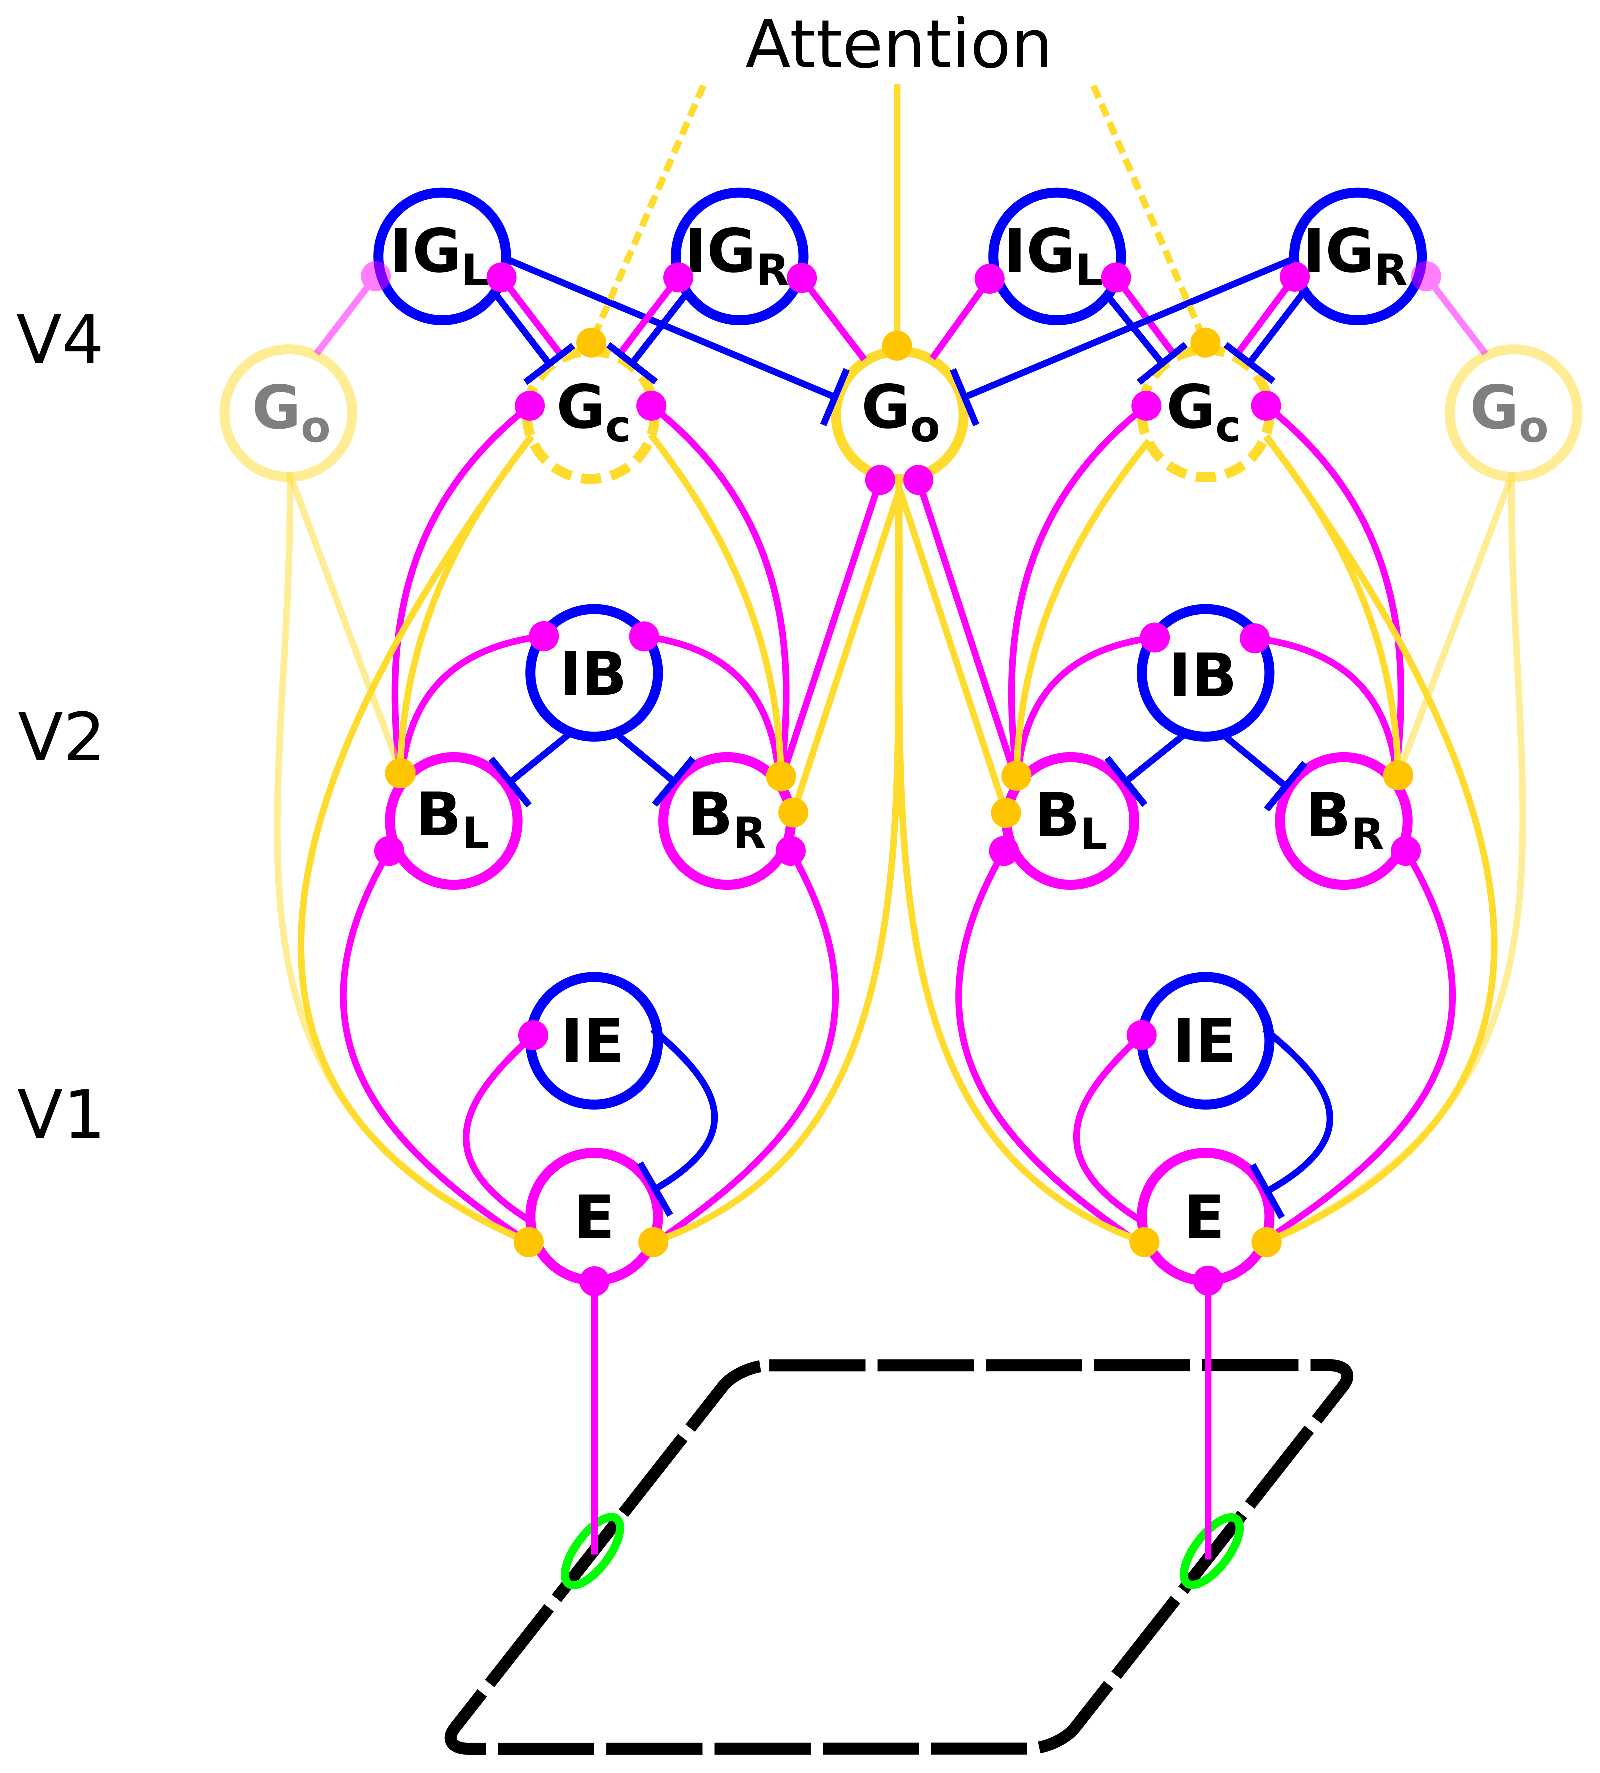
\includegraphics[width=0.75\textwidth]{Contour/figs/Fig1.eps}
\makeatletter
\let\@currsize\normalsize
% simplify caption
\caption[Structure of the grouping model network]{Structure of the model network. Each circle stands for a population of neurons with similar receptive fields and response properties. Magenta, blue, and orange lines represent feedforward excitatory, lateral inhibitory, and feedback excitatory projections, respectively.
\comment{Edges and other local features of a figure (black dashed
parallelogram) activate edge cells (E), whose receptive fields are   shown by green ellipses. Edge cells project to border ownership cells (B) that have the same preferred orientation and retinotopic position as the E cells they receive input from. However, for each location and preferred orientation there are two B cell populations with opposite side-of-figure preferences, in the example shown $B_{L}$ whose neurons respond preferentially when the foreground object is to the left of their receptive fields and $B_{R}$ whose members prefer the foreground to the right side of their receptive fields.\ E cells also excite other E cells with the same preferred orientation (connections not shown),  as well as a class of inhibitory cells (IE) which, in turn, inhibit E cells of all preferred orientations at a given location (only E cells of one preferred orientation are shown). B cells have reciprocal, forward excitatory and feedback modulatory connections with two types of grouping cells, $\rm G_c$ and $\rm G_o$, which integrate global context information about contours and objects, respectively. E cells also receive positive modulatory feedback from these same grouping cells. Opposing border ownership cells compete directly {\em via} IB cells and indirectly {\em via} grouping cells, which bias their activity and thus generate the response differences of opposing border ownership selective neurons. G cell populations also directly excite
inhibitory grouping cells (IG; again with the indices L and R), which inhibit $\rm G_c$ cells nonspecifically and $\rm G_o$ cells in all orientations except the preferred one.}
Top-down attention is modeled as input to the grouping cells and can therefore either be directed towards objects (solid lines) or contours (dashed lines) in the visual field (top).}
\label{Fig:anatomy}
\end{figure}

\section{Methods} 
\label{sec:model}

\subsection{Model structure}

The model consists of areas V1, V2, and V4
(Figure~\ref{Fig:anatomy}). The model receives input from a
binary-valued orientation map with four orientations
($0, \pi/4, \pi/2,$ and $3\pi/4$ relative to the horizontal). The
input signal is first represented in V1 and then propagated to V2 and
V4 by feedforward connections. Area V4 provides feedback to lower
areas (see \hyperref[sec:appendix_eq]{Appendix A} for equations). Neurons in higher
areas have larger RFs and represent the image at a coarser
resolution. RF sizes in area V4 are four times larger than the RF
sizes in V2, which, in turn, are twice as large as the sizes in V1.

To achieve contour integration, we implement excitatory lateral
connections between V1 edge (E) cells with the same orientation
preference. These connections are similar to the local association
fields used in other models~\citep{Li98,Piech_etal13}. Background
suppression is carried out through a separate population of inhibitory
(IE) cells. The input from V1 activates populations of border
ownership (B) cells in V2 with identical orientation preferences and
opposing side-of-figure preferences. A combination of lateral
connections within V2 and feedback connections from V4 (described
below) is used to generate border ownership selectivity. Inhibitory
(IB) cells in V2 cause competition between B cells at the same
location and same orientation preference but opposite side-of-figure
preference.

\begin{figure}[t]
\centering
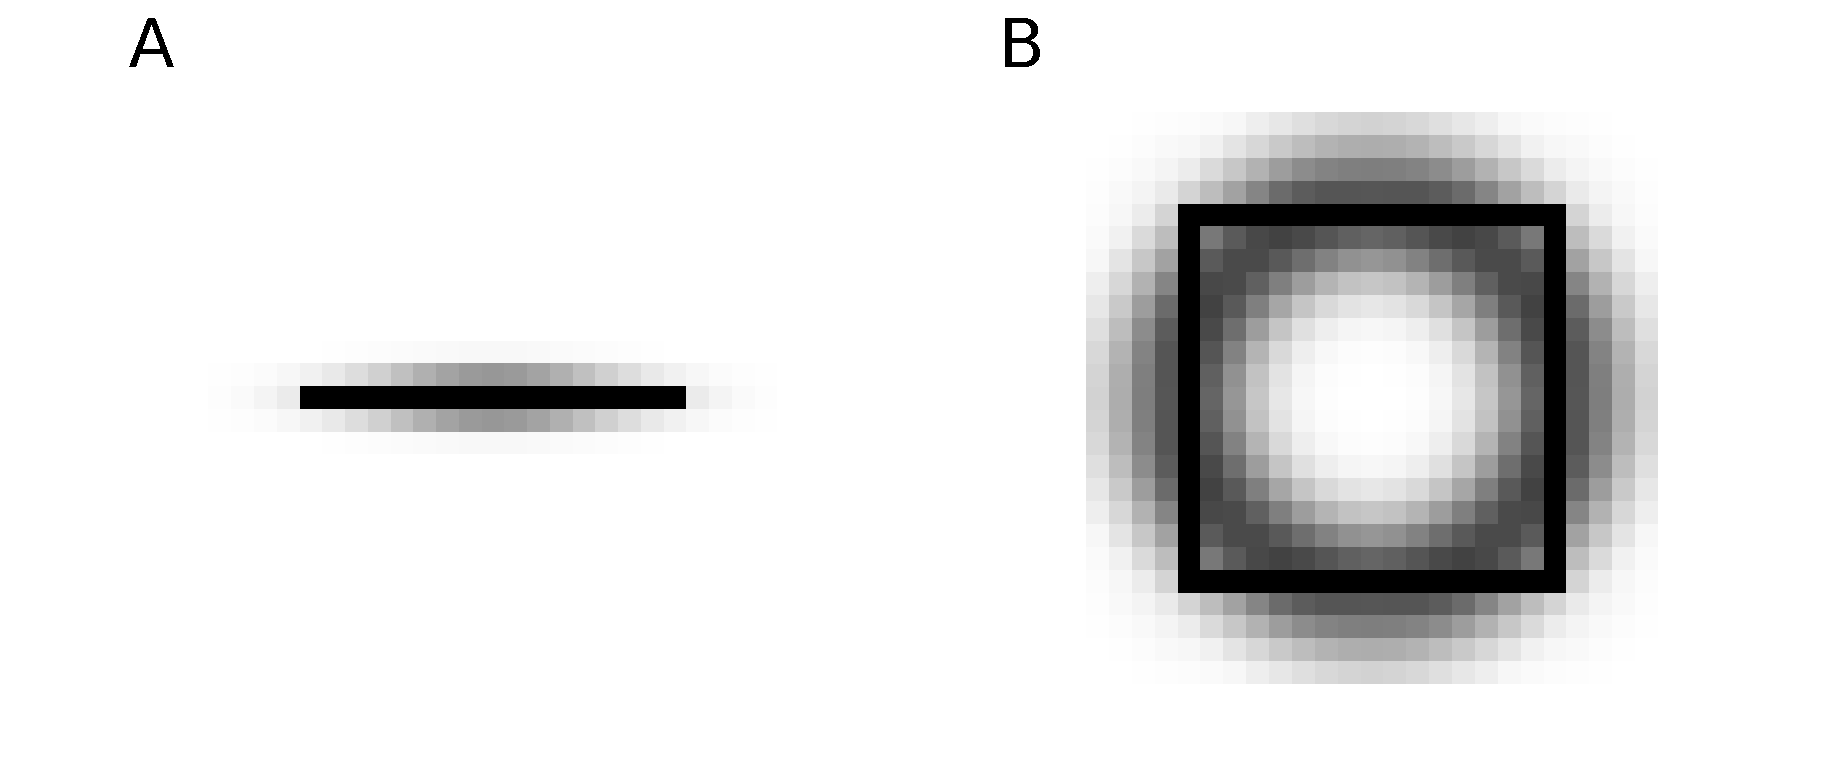
\includegraphics[width=\textwidth]{Contour/figs/Fig2.eps}
\makeatletter
\let\@currsize\normalsize
\caption[Contour and object grouping cell receptive fields]{Spatial distribution of border ownership cell to grouping cell connectivity; darker pixels indicate stronger connection weights. A) Contour grouping neurons integrate features along oriented contours (horizontal line shown in black), emphasizing the Gestalt principle of good continuation. B) Object grouping neurons integrate features in a co-circular pattern (square figure shown in black), emphasizing the Gestalt principles of convexity and proximity.} 
\label{Fig:BG_projections}
\end{figure}

In V4, two different types of grouping cells exist. Contour grouping cells ($\rm G_c$) integrate local edge information and are selective for oriented contours (Figure~\ref{Fig:BG_projections}A). Object grouping cells ($\rm G_o$) are sensitive to  co-circular arrangements of edges which combines
features of the Gestalt laws of good continuation, convexity of contour, and compact shape
(Figure~\ref{Fig:BG_projections}B). Competition between separate contours and objects is carried out by a population of inhibitory (IG) cells. Grouping ($\rm G_c$ and $\rm G_c$) cells project back exactly to those B cells from which they receive input, and also to the E cells which are co-activated with B cells. This feedback enhances the activity of E cells along contours and biases the competition between B cells to correctly assign border ownership along object boundaries. Importantly, feedback connections are modulatory, rather than driving, such that the feedback does not modify activities of cells that do not receive sensory input, as for instance through glutamatergic synapses of the NMDA type \citep{Wagatsuma_etal16a}.

To model the effect of object-based attention, we assume that areas higher than V4 provide additional excitatory input to grouping cells, whose activity represents the presence of objects or contours, as shown in Figure~\ref{Fig:anatomy}. This attentional input is driving but relatively weak; we select its strength as 7\% of that of the driving input to the sensory (E) cells. We also model the effect of a lesion in V4 that removes the feedback completely by setting the weight of
feedback connections from V4 to lower areas  to zero.

Our approach is an extension of the proto-object-based model of perceptual organization proposed by \cite{Mihalas_etal11b}. Different from their approach, we include a new population of contour grouping neurons to explain recent results on cortico-cortical interactions during contour integration~\citep{Chen_etal14}. As a result, top-down attention in our model can either be directed to grouping neurons representing contours or objects. Our model is also able to reproduce
the time course of neural responses in different visual areas, while the \cite{Mihalas_etal11b} model only explains mean neural activities. In order to create more complex input stimuli, we also
increased the number of model orientations from two to four. As a simplification to their model, we only include one scale of grouping neurons since we focus on mechanisms that do not require multiple
scales.

\subsection{Model implementation}
\label{sec:implementation}

Model neuronal populations (usually referred to as ``neurons'' in the
following) are represented by their mean activity (rate coding).  The
activity is determined by a set of coupled, first-order nonlinear
ordinary differential equations which was solved in MATLAB (MathWorks,
Natick MA) using standard numerical integration methods.  The mean
firing rate is necessarily positive, therefore units are simple
zero-threshold, linear neurons which receive excitatory and inhibitory
current inputs with their dynamics described by,
\begin{equation}
\label{eq:1}
\tau f'(t) = -f + \left[ \sum W \right]_{+}
\end{equation}
where $f$ represents the neuron's activity level and $\tau$ its time
constant, chosen as $\tau$ = $10^{-2}$ s for all neurons. The sum is
over all $W$ which are the neuron's inputs,
$f'$ is the first derivative of $f$ with respect to
time, and $[\,]_{+}$ means half-wave rectification.

All simulations were performed on a 300-core CPU cluster running Rocks
6.2 (Sidewinder), a Linux distribution intended for high-performance
computing.  A total of 100 simulations were performed for each
experimental condition, and our results are based on the mean neural
activities averaged over these simulations with different randomly
selected stimulus noise patterns, see sections~\ref{sec:contour_exp}
and~\ref{sec:FGO}.

To constrain our model parameters, we used two sets of
neurophysiological data. The first comes from recent contour grouping
results~\citep{Chen_etal14}, and our model was able to largely
reproduce the magnitude and time course of contour integration at both
the V1 and V4 levels. The second set of results comes from studies on
border ownership coding~\citep{Qiu_etal07}, specifically the vector
modulation index at the V2 level (see section~\ref{sec:vmi}) in the
presence and absence of attention. In order to fit the model
parameters, we started from the parameters given by
\cite{Mihalas_etal11b}, and modified them to fit the larger body of
experimental results to include contour integration, border ownership
selectivity, and attentional selection.

\begin{figure}[t]
\centering
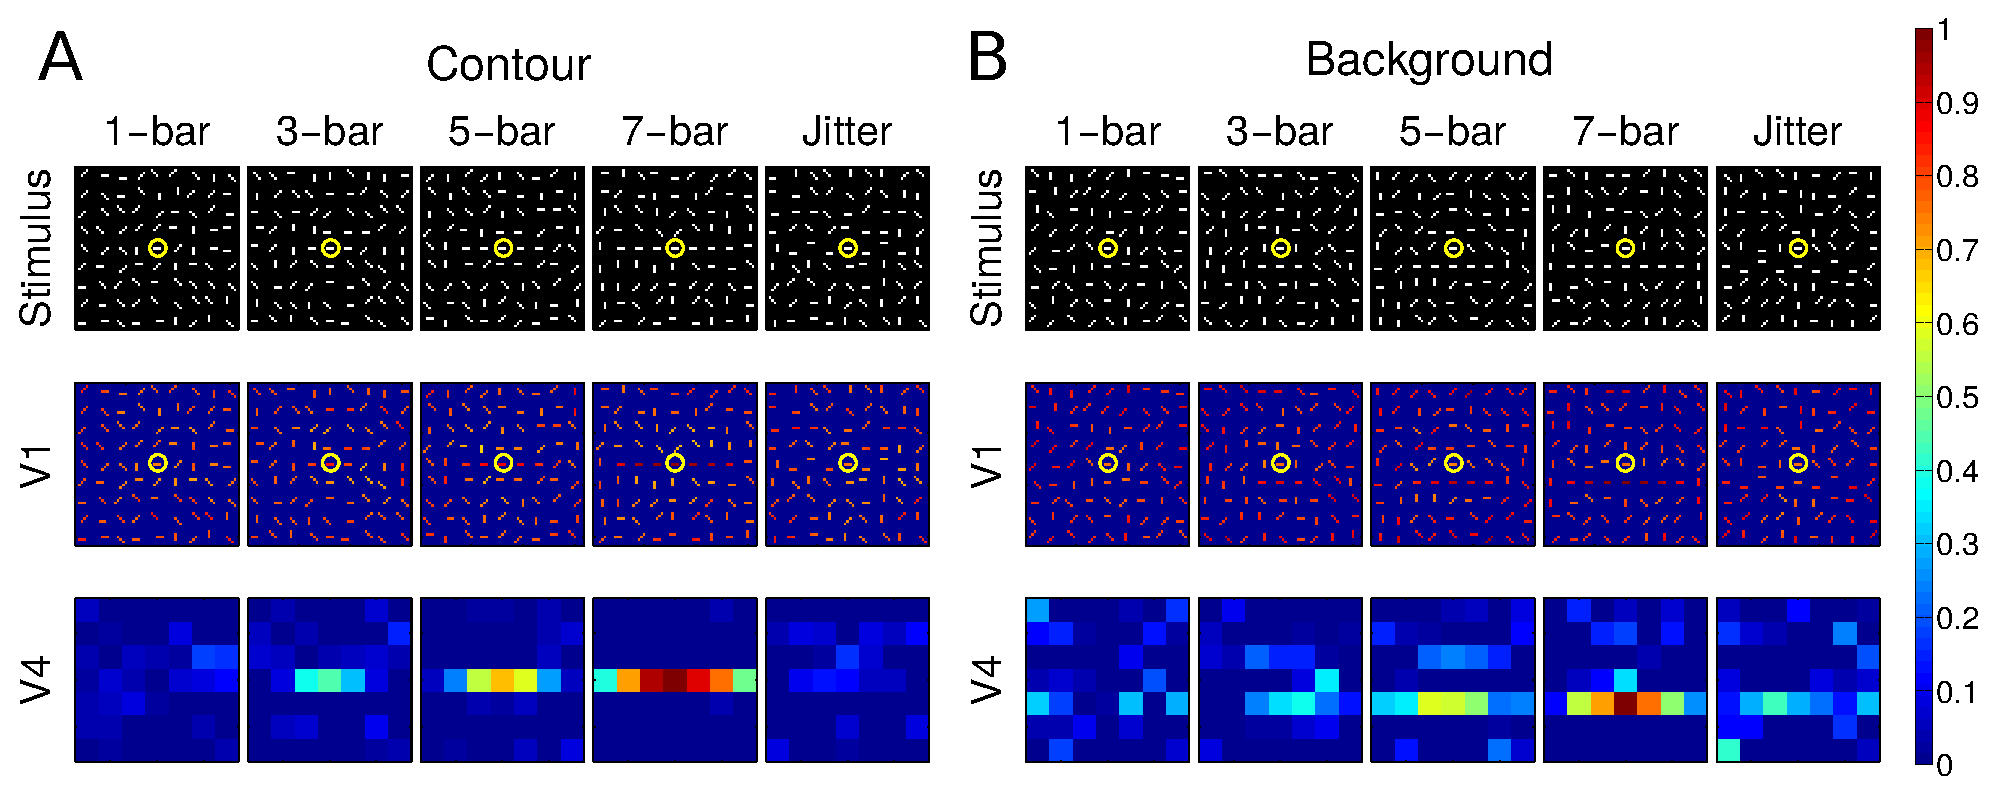
\includegraphics[width=\textwidth]{Contour/figs/Fig3.eps}
\makeatletter
\let\@currsize\normalsize
\caption[V1 and V4 population responses to contours]{Normalized V1 $E$ cell and V4 $G_c$ cell population responses to contours of varying lengths in either the contour (A) or the background (B) condition. In (A), the ``recorded'' neuron is on the contour; in (B), it is offset from the contour. The top row shows stimuli, the second and third rows show activity in model areas V1 and V4, respectively. Yellow circles mark the RFs of the V1 neurons whose activity is shown in Figure~\ref{Fig:Neural_responses}. 
\comment{Activity from model area V2 is not shown because a single contour does not produce clear border ownership selectivity, and the activity in V2 is essentially the same as that in V1, but with reduced spatial resolution due to the lower number of neurons.}
Columns in each condition show, from left to right, increasing contour length, with the right-most column showing a jittered stimulus configuration (see text). Neural activity is color coded and normalized to the 7-bar stimulus in both contour and background conditions, with warmer colors representing higher activity (see color bar at right).}
\label{Fig:Contour_Results}
\end{figure}

\subsection{Contour integration experiments} 
\label{sec:contour_exp}

For the contour integration experiments reported by
\cite{Chen_etal14}, awake behaving monkeys were trained to perform a
two-alternative forced-choice task using two simultaneously presented
patterns, one containing a contour embedded in noise and one that was
noise only (see Figure~\ref{Fig:Contour_Results} for examples).  The
patterns were composed of $0.25^{\circ}$ by $0.05^{\circ}$ bars
distributed in $0.5^{\circ}$ by $0.5^{\circ}$ grids.  The diameter of
the patterns was $4.5^{\circ}$, and the number of bars in the embedded
contour was randomly set to 1, 3, 5, or 7 bars within a block of
trials in order to control the saliency of the contour.  To obtain a
reward, the monkey had to saccade to the pattern containing the
contour, with the location of the stimulus containing the contour as
well as the number of collinear bars making up the contour changing
between trials.  When the number of bars was set to 1, both presented
stimuli were noise patterns, and the monkey had to guess randomly with
a probability of 50\%.  While the animals were performing the task,
simultaneous single- or multi-unit recordings were made in area V1 and
V4 neurons with overlapping receptive fields.

We modeled these experiments by creating visual stimuli contained in a
$4.5^{\circ}$ by $4.5^{\circ}$ area as in the~\cite{Chen_etal14}
study. This area was projected onto a V1 layer of $64 \times 64$
neurons, each with a receptive field size of $\sim0.7^{\circ}$ so the
receptive fields overlapped ten-fold at each location in the visual
field.  We divided the input field into a $9 \times 9$ grid (each grid
point at the center of a $0.5^{\circ}$ by $0.5^{\circ}$ area) and we
placed at each grid location a stimulus bar 
consisting of three adjacent pixels, corresponding to a size
$\sim0.21^{\circ}$ by $\sim0.07^{\circ}$. 
Each stimulus bar had one of four orientations, $0, \pi/4, \pi/2,$ or
$3\pi/4$.  As in the experiment, contours consisted of 1, 3, 5, or 7 adjacent
stimulus bars. We always positioned the contour at the center of the
visual field, and we changed the length of the contour by adding bars
to either end of the contour. We ``recorded'' from the V1 receptive
field that was at the center of the stimulus (marked by the yellow
circles in Figure~\ref{Fig:Contour_Results}), as well as from the
corresponding V4 neuron.  Due to their size, V4 receptive fields
basically enclosed the entire contour.

\subsection{Figure-ground segregation experiments} 
\label{sec:FGO}

For the figure-ground segregation experiments~\citep{Zhou_etal00,
  Qiu_etal07, Zhang_vonderHeydt10}, awake, behaving monkeys were
trained on a fixation task.  Receptive fields of each recorded neuron
in areas V1 and V2 were first mapped to determine the optimal stimulus
properties for that neuron. Afterwards, in some experiments, a square
shape was presented on a uniform gray background with one edge of the
square centered on the receptive field of the neuron at the neuron's
preferred orientation.  In other experiments (results shown in
Figures~\ref{Fig:Overlap_Square_exp_model}
and~\ref{Fig:Overlap_Square}) the stimulus consisted of two partially
overlapping squares, and again the receptive field of the recorded
neuron was centered at its preferred orientation on one edge of one of
the squares.  The size of the square varied between experiments but it
was always chosen such that the closest corner was far away from the
classical receptive field of the recorded neuron. The square was
presented in two positions between which it was ``flipped'' along the
long axis of the neuron's receptive field. For instance, if the
preferred orientation was vertical, the square was presented either to
the left or the right of the cell's receptive field (we used this
example in the choice of the indices in Figure~\ref{Fig:anatomy}).
The difference in the firing rate of the neuron for when the square
appears on one side versus the other side is known as border ownership
selectivity. Importantly, in all stimulus conditions, local contrast
within the receptive field of the neuron remained the same between
these two conditions; only global context information about the side
of the square changed, so the neuron had to integrate information from
outside its classical receptive field.

We modeled these experiments by creating visual stimuli that were
projected onto the V1 layer. The input to the simulation was 
either a single square of a size that maximally activated $\rm G_o$ grouping cells of
the size chosen in our model, or two partially overlapping squares, as shown in
Figure~\ref{Fig:Overlap_Square}, with each of these squares having the same
optimal size. In more general models \citep{Craft_etal07,Mihalas_etal11b,Russell_etal14},
grouping cells of many scales are present, covering the range of possible objects in the
input. We calculated border ownership selectivity at the V2 level
using the vector modulation index defined in section~\ref{sec:vmi}.
In order to create noisy versions of the single square image
(Figure~\ref{Fig:Square}, bottom row), we followed a
similar approach as in the contour integration experiments.  We again
divided the visual field into a $9 \times 9$ grid and we positioned
horizontal and vertical bars at specific grid points to generate a
square. We then placed a stimulus bar at all other grid points, with
their orientations randomly chosen from four possibilities,
$0, \pi/4, \pi/2,$ and $3\pi/4$.

\subsection{Quantitative assessment of border ownership selectivity:
  vector modulation index}
\label{sec:vmi}

The strength of border ownership selectivity was quantified using the
vector modulation index, introduced by~\cite{Craft_etal07} and defined
by the expression 
\begin{equation}
\label{eq:2}
\vec{v}(x,y) = m_{\hat{\imath}}(x,y)\hat{\imath} + m_{\hat{\jmath}}(x,y)\hat{\jmath}
\end{equation}
where $\hat{\imath}$ and $\hat{\jmath}$ are unit vectors along the horizontal and vertical image
axis, respectively, and the components $m_{\hat{\imath}}(x,y)$ and $m_{\hat{\jmath}}(x,y)$ are the usual modulation indices along their respective axes, defined as
\begin{equation}
\label{eq:3}
\begin{split}
	m_{\hat{\imath}}(x,y) = \frac{\sum_{\theta}
        B_{\theta}(x,y)\cos\theta}{\sum_{\theta}
                \left|B_{\theta}(x,y)\cos\theta\right|} \\
	m_{\hat{\jmath}}(x,y) = \frac{\sum_{\theta}
        B_{\theta}(x,y)\sin\theta}{\sum_{\theta}
                \left|B_{\theta}(x,y)\sin\theta\right|}
\end{split}
\end{equation}
where $B_{\theta}(x,y)$ is the border ownership signal (difference between
the activities of the two opposing B neurons) at the preferred
orientation $\theta$ at position $(x,y)$, and $\theta$ runs over all
angles taken into account in the model 
(four directed orientations in our case, namely $0, \pi/4, \pi/2,$
and $3\pi/4$, each with both side-of-figure preferences). 
Vertical bars in the sums in the denominators indicate absolute values.

Both components in Eq.~\ref{eq:3} are limited to values between +1 and
-1. For the x-component, for instance, a positive value of
$m_{\hat{\imath}}(x,y)$ signifies that the figure is to the right of
position (x,y) and a negative value signifies that the figure is to
the left. Its absolute value indicates the ``strength'' of the
border-ownership signal, with zero being equivalent to ambivalence
between left and right. Corresponding comments apply to the
y-component, $m_{\hat{\jmath}}(x,y)$, regarding the figure's position
upward or downward of (x,y). The direction of the vectorial modulation
index $\vec{v}(x,y)$ defined in Eq.~\ref{eq:2} indicates the position
of the foreground figure in the two-dimensional image plane relative
to the point (x,y). For instance, positive values in both components
[$m_{\hat{\imath}}(x,y) > 0$, $m_{\hat{\jmath}}(x,y) > 0$] indicate
that the figure is located upwards and to the right of (x,y).

\section{Results}
\label{sec:results}

\subsection{Contour enhancement in V1 and V4}
We examined contour-related responses in our model using visual
stimuli composed of collinear bars among randomly oriented bars
(Figure~\ref{Fig:Contour_Results}), closely matching the stimuli used
in the physiological experiments by~\cite{Chen_etal14}. The number of
collinear bars constituting an embedded contour was set to either 1,
3, 5, or 7 bars, determining the length of the embedded contour, which
also controlled its saliency.  When the number of collinear bars was
one, the stimulus was identical to a noise pattern. We compared the
activity of model neurons whose RFs are centered on the contours or in
the noise background (but close to contours) with that obtained in the
analogous positions during neurophysiological recordings.

V1 responses were split into those of neurons on contour sites
(C-sites) and background sites (B-sites). For contour sites
(Figure~\ref{Fig:Contour_Results}A), the embedded contour was centered
on the RF of a neuron with a preferred orientation matching that of
the contour. For background sites, the contour was laterally placed
0.5$^{\circ}$ away from the RF center of the recorded neuron, and a
background bar was placed in the RF
(Figure~\ref{Fig:Contour_Results}B), with the contour orientation
again matching the preferred orientation of the recorded neuron.
Both V1 and V4 neurons along the contour showed increased activity with contour length. Neurons on the background showed increased suppression with contour length.
Correspondingly, we show in Figure~\ref{Fig:Neural_responses} the
responses of neurons whose preferred orientations align with the
contours (yellow circles in Figure~\ref{Fig:Contour_Results}).

\begin{figure}[t!]
\centering
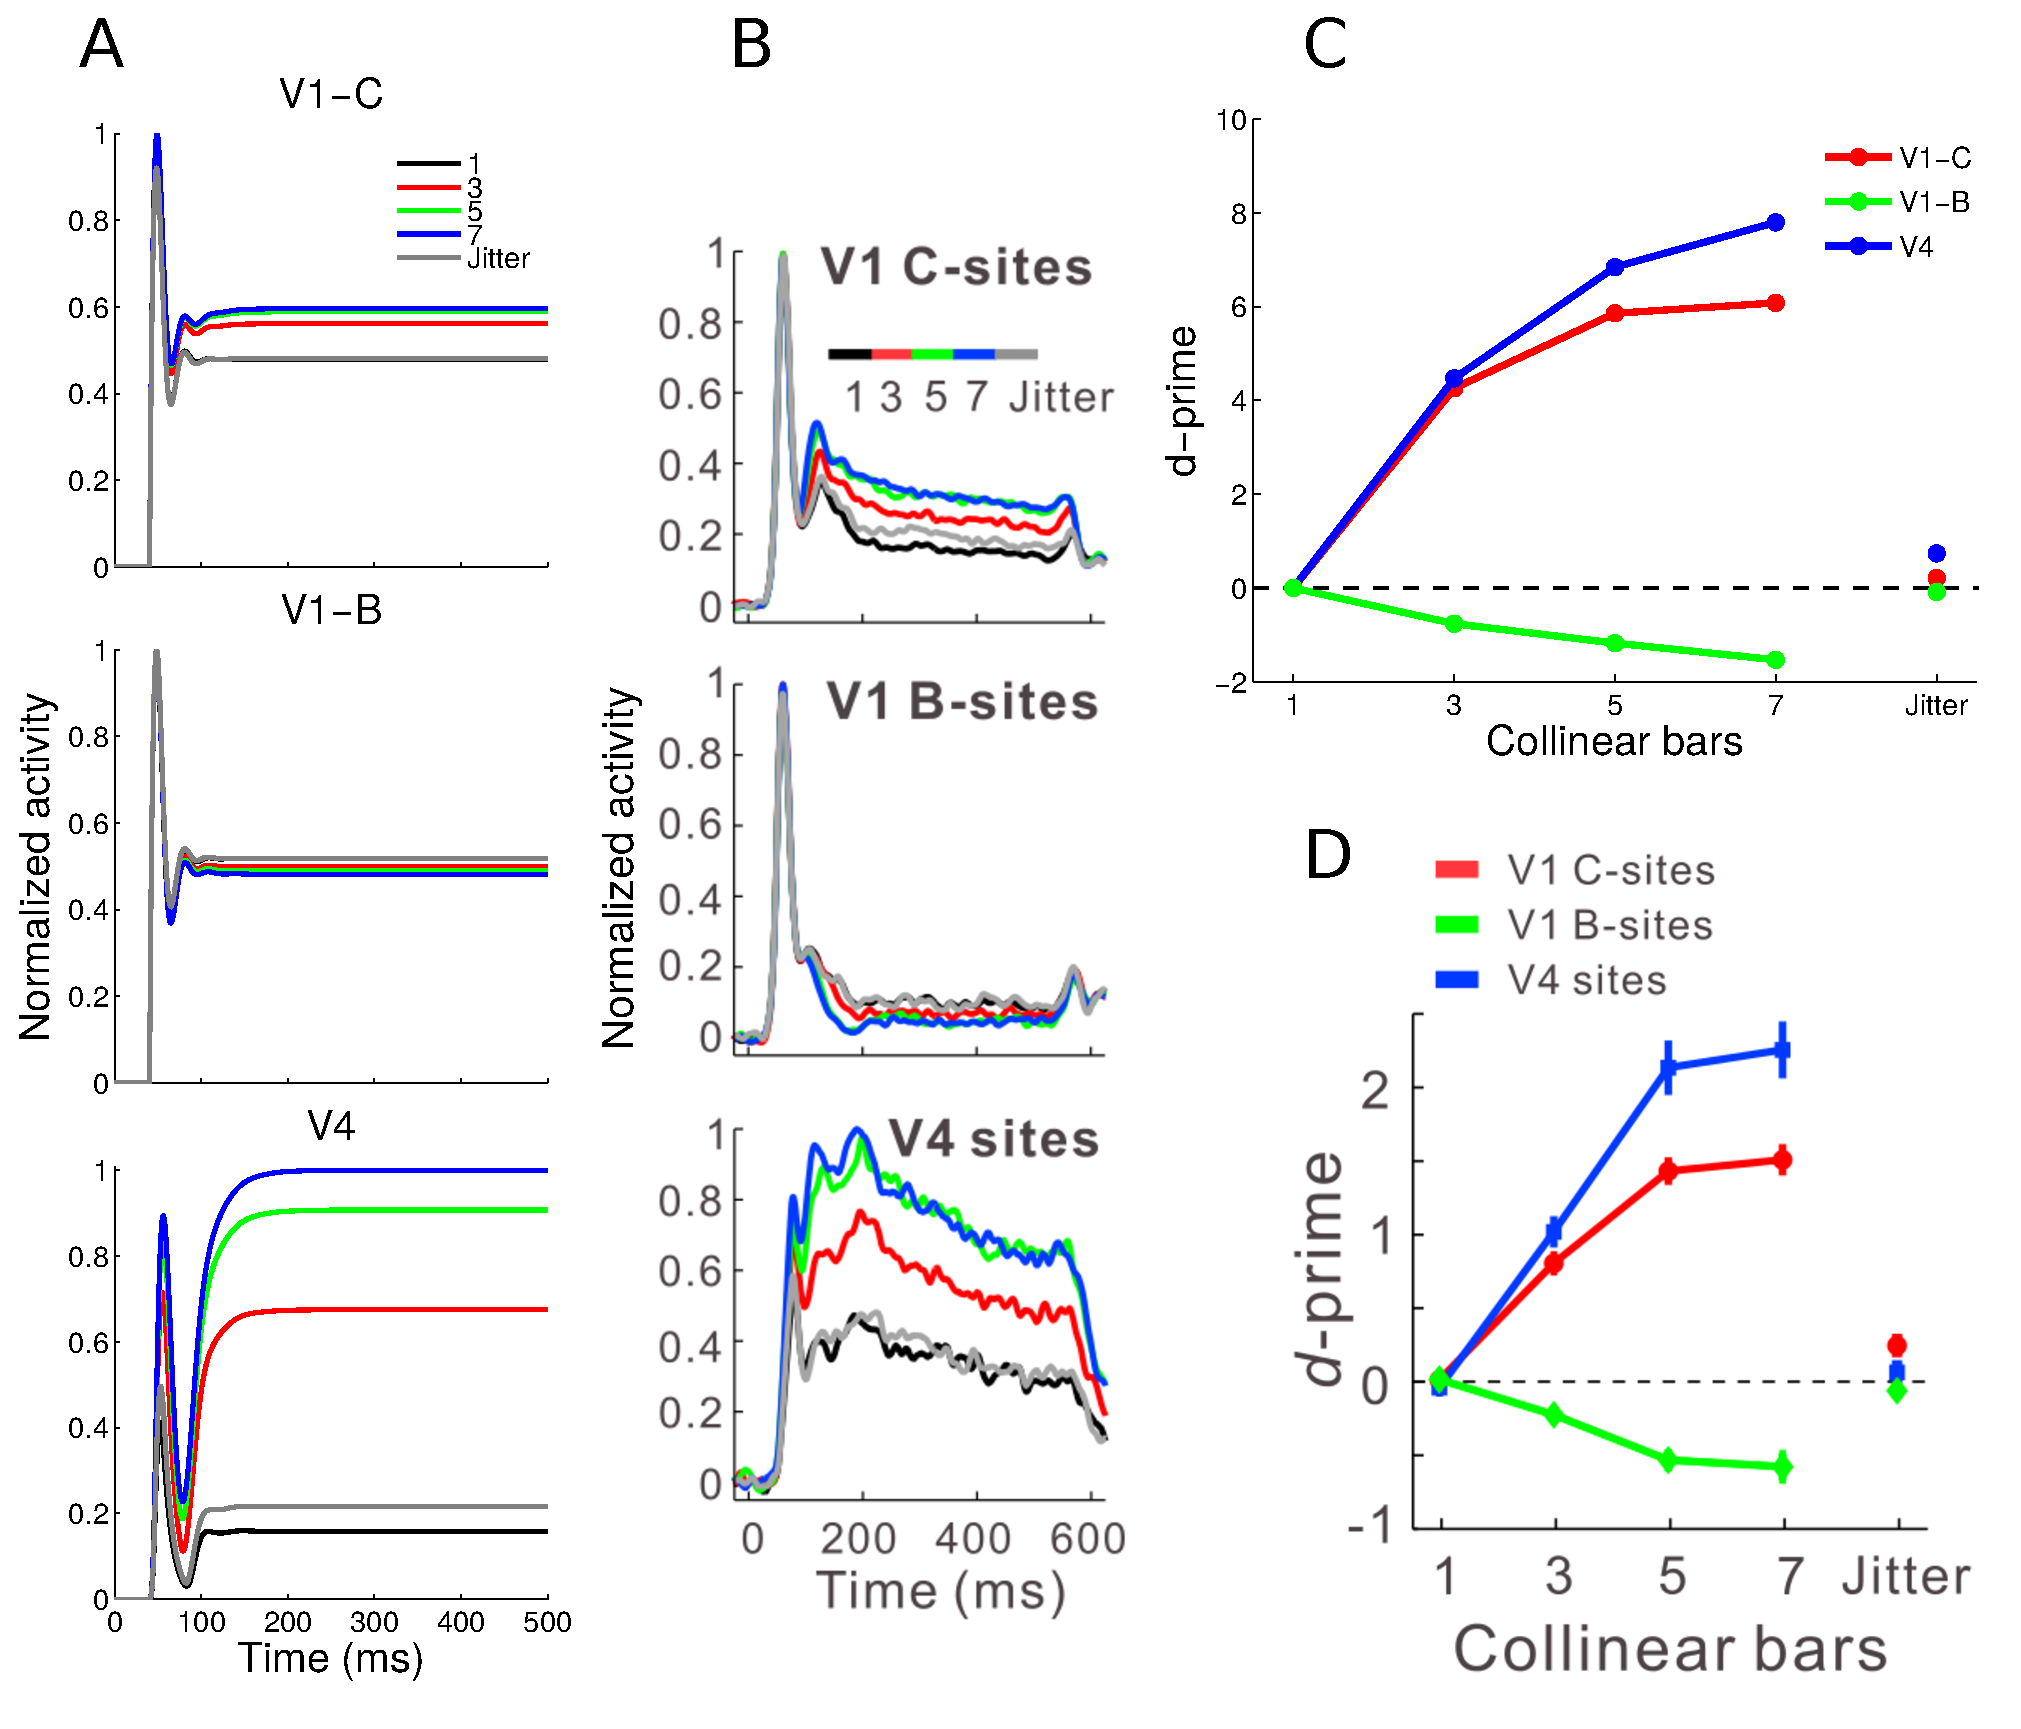
\includegraphics[width=0.75\textwidth]{Contour/figs/Fig4.eps}
\makeatletter
\let\@currsize\normalsize
\caption[Time course of neural activity in V1 and V4 and the contour-response d-prime measure]{Normalized V1 $E$ cell (contour and background sites) and V4 $G_c$ cell neuronal activity and contour-response $d'$ to contours of varying lengths. (A) V1 contour (top) and background (middle) sites and V4 sites (bottom).
%showed facilitation followed by saturation with increasing contour length (see legend). V1 background sites showed greater suppression with longer contours. 
The jitter condition involved a 7-bar pattern where each bar was laterally offset to disrupt collinearity. (B) Corresponding experimental observations showing normalized and averaged PSTHs from the~\cite{Chen_etal14} study. (C) Contour-response $d'$ was higher for the V4 sites compared to the V1 contour sites.
%, and was facilitated by  increasing contour length. 
V1 background sites had increasingly  negative $d'$ with longer contours.
%, indicating background suppression. The jitter condition reduced the absolute value of the $d'$ values to close to zero, making it similar to the baseline noise condition.
(D) Corresponding experimental observations, showing the mean contour-response $d'$ from the~\cite{Chen_etal14} study. Panels B and D are modified from Figure~2 of~\cite{Chen_etal14}. All model results (neural responses and contour-response $d'$) are averages for a single neuron over 100 simulations.}
\label{Fig:Neural_responses}
\end{figure}

Except for an input delay of 40ms corresponding to the duration of
visual processing from the retina to V1, we did not explicitly model
any time delays in the feedforward or feedback connections of
our model, as we were not attempting to reproduce 
any specific latency effects.
Nevertheless, our model generally reproduced the dynamics of neural
responses to contours in both V1 and V4 observed in the
\cite{Chen_etal14} experiment (Figure~\ref{Fig:Neural_responses}A).
The most salient feature of the neuronal responses is that the levels
of sustained activity differ based on the number of bars in the
embedded contour. This is observed both for contour sites and for
background sites but, importantly, this effect went in opposite
directions for these two cases.  As the number of collinear bars
increased from one to seven, V1 contour sites centered on the contour
showed increased activity, with response saturation after five
bars. In contrast, V1 background sites that were offset from the
embedded contour showed a decrease in activity with increasing number
of bars in the background (response suppression). Similar to V1
contour sites, V4 sites showed saturating responses with increasing
contour lengths (Figure~\ref{Fig:Neural_responses}A, bottom).  These
results were qualitatively similar to those obtained in
the~\cite{Chen_etal14} experiments which are reproduced in
Figure~\ref{Fig:Neural_responses}B (their Figure~2A).

The model data also showed strong onset transients in both (contour
and background) V1 populations (Figure~\ref{Fig:Neural_responses}A,
top and center), again in good agreement with experimental results
(Figure~\ref{Fig:Neural_responses}B, top and center). Transients in V4
neurons were weaker, in both model and experimental data, and nearly
absent in the experimental data (though not the model) for longer
contours (Figure~\ref{Fig:Neural_responses}B, bottom).
The transient peak observed in the model results
is due to a sharp suppression of the activity level for a short
($<50$ms) period which is not observed in the empirical data. We
believe that this suppression is due to the  strong inhibition at the
V4 level between G and IG cells, without equivalent
excitation between different G cells.

Following~\cite{Chen_etal14}, 
we quantitatively analyzed the contour responses using the d-prime
$(d')$ metric from signal detection theory~\citep{Green_Swets66}, which
quantifies the difference in distributions of mean neuronal firing
rates between a contour pattern and the noise pattern integrated over
the whole interval shown in Figure~\ref{Fig:Neural_responses}A,B, \ie
0-500 ms.  Neuronal responses to the 1-bar pattern (the noise pattern)
were the baseline for examining contour-related responses in V1 and
V4, this pattern therefore had a contour-response $d'$ of zero. The
contour-response $d'$ increased with contour length for both the V1
contour and V4 sites, and $d'$ decreased with contour length for the V1
background sites, Figure~\ref{Fig:Neural_responses}C.

The agreement between model (Figure~\ref{Fig:Neural_responses}C) and
experimental results (Figure~\ref{Fig:Neural_responses}D) is striking.
One difference we note is that the absolute values of all model $d'$
substantially exceeded the corresponding experimental values. 
This is to be expected since no noise was included in the model 
(other than the random orientation of input
stimulus bars which is also present in the experimental approach)
while there are surely multiple sources of noise in the biological
system. We have not thoroughly investigated this question but it is
likely that addition of noise to the model will decrease the $d'$
values.

At first sight, it seems possible that 
V4 neurons respond with a higher firing rate to longer contours than
to shorter ones simply as a consequence of 
the large size of RFs in V4. 
In this view, the enhanced responses in V4 with increasing contour
length is due to the spatial summation of many bars
within the RF at the optimal orientation,
independent of their precise location in the RF. 
To  investigate this possiblity,
~\cite{Chen_etal14} introduced a ``jitter'' condition to the 7-bar
contour, where alternating collinear bars were laterally offset 
by a small amount (much less than the receptive field size)
in order to disrupt the collinearity of the original contour. They
showed that jittering disrupted the 
contour integration process and reduced the neural responses in V1
and V4 close to baseline levels (Figure~\ref{Fig:Neural_responses}B,
gray lines). We found the same result in our model,
Figure~\ref{Fig:Neural_responses}A, gray lines.  Furthermore, in the
jitter condition, contour-response $d'$ approached baseline for the
V1 and V4 sites, as shown in the rightmost points for
Figure~\ref{Fig:Neural_responses}D for experimental data and
Figure~\ref{Fig:Neural_responses}C for model results. In both cases,
no substantial difference between the jitter condition and the
baseline noise condition was observed.

We also investigated the orientation and position dependence of
contour-related responses in V1 and V4, and found close agreement of
our model results with experimental data~\citep{Chen_etal14}. Due
to space constraints, these results are presented in \hyperref[sec:appendix_fig]{Appendix A}.
%Supplementary Material. The results for V4 are presented in Supplementary Figure~\ref{Fig:V4_total} and the results for V1 are presented in Supplementary Figure~\ref{Fig:V1_total}.

\begin{figure}[t]
\centering
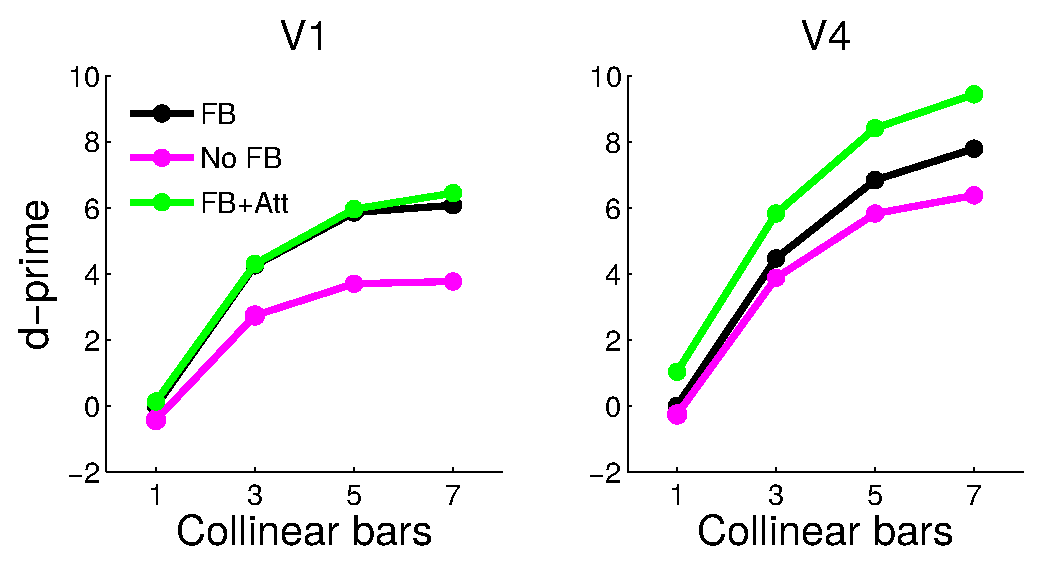
\includegraphics[width=\textwidth]{Contour/figs/Fig5.eps}
\makeatletter
\let\@currsize\normalsize
\caption[Model prediction of the effect of feedback and attention on contour-response d-prime]{Contour-response $d'$ in V1 $E$ cells (A) and V4 $G_c$ cells (B) for the model with (green) and without attention (black), and for the model with feedback removed (magenta). Attention strongly increased
contour-response $d'$ in V4 (B), while the lack of feedback strongly
decreased contour-response $d'$ in V1 (A).}
\label{Fig:FB_att}
\end{figure}

\subsection{The role of feedback and attention in contour grouping}   

While different forms of attention exist that can be flexibly used for
different tasks, we choose here to focus only on the mechanisms of
object-based attention
\citep{Egly_etal94,Scholl01,Kimchi_etal07,Ho_Yeh09}.  We postulate
that attention to objects acts at the level of grouping neurons, in
agreement with the~\cite{Mihalas_etal11b} model.  As shown in that
study, modulation of the activity of grouping cells bypasses the need
for attentional control circuitry to have access to detailed object
features.  Instead, grouping neurons are used as ``handles'' of the
associated objects and it is in their interaction with feature-coding
neurons that features are assigned to objects. One of the consequences
of this mechanism is that the spatial resolution of attentional
selection is coarser than visual resolution since the smallest
``unit'' of spatial attentional deployment is the size of the
receptive (and projective) field of grouping cells, which is
considerably larger than the receptive fields of feature-coding
neurons at the same eccentricity. Behavioral results show strong
evidence in favor of this coarse attentional
resolution~\citep{Intriligator_Cavanagh01}.

In our model, attention can be directed to objects, including
contours. For the contour integration experiments, this is implemented  as a top-down input to all contour grouping neurons at the attended location.
As we have seen before (Figure~\ref{Fig:Neural_responses}), $d'$ in V1
and V4 populations increases with the number of collinear bars, even
in the absence of attention.  In addition, we now show that attention
increases the contour-response $d'$ for both V1 and V4 neurons, with
the additive effect being much larger in V4 than in V1
(Figure~\ref{Fig:FB_att}). For the 7-bar contours, attention increases
the contour-response $d'$ in V1 from 6.08 to 6.66 and in V4 from 7.80
to 11.59. This is consistent with findings that attention has a much
larger effect on higher-level neurons compared to early sensory
neurons~\citep[review:][]{Treue01}.

One of the advantages of computational modeling is that it allows the
study of scenarios that are difficult to implement empirically.
One question that is difficult to answer experimentally is how removal of
feedback 
from V4 to lower visual areas
would change neuronal responses in V1 and V4, structures that
are known to be connected bidirectionally.
While it is possible to study the influence of feedback on V2 (and
other areas) by cooling \citep{Hupe_etal98} or pharmacological
inactivation \citep{Jansen_etal12} of area V4, such manipulations only
allow limited control of the effect on multiple brain structures. In
contrast, a computational model allows the study of interactions
between different areas with perfect control. In the model, 
we can eliminate all feedback from area V4 simply by ``lesioning'' the
connections from the grouping neurons to the V2 and V1 neurons
(setting their strength to zero), thus turning the model into a
feedforward network.  We found that this has the opposite effect of
applying attention on the $d'$ metric: the decrease in contour
response $d'$ was much larger in V1 compared to V4. Removing feedback
reduced the 7-bar contour-response $d'$ in V1 from 6.08 to 3.77, and
in V4 from 7.80 to 6.38 (Fig.~\ref{Fig:FB_att}). We note that the
contour-response $d'$ in V1 is above zero even without feedback from
grouping neurons because of the contribution of local excitatory
connections to contour integration.  This asymmetric effect in contour
response $d'$ in the two areas (V1 and V4) may point to the different
roles of feedforward and feedback processing in early vision. We are
not aware of any experimental manipulations that completely remove
feedback from area V4 without changing the circuitry in other ways, so
our results are a prediction awaiting experimental falsification.

\begin{figure}[t]
\centering
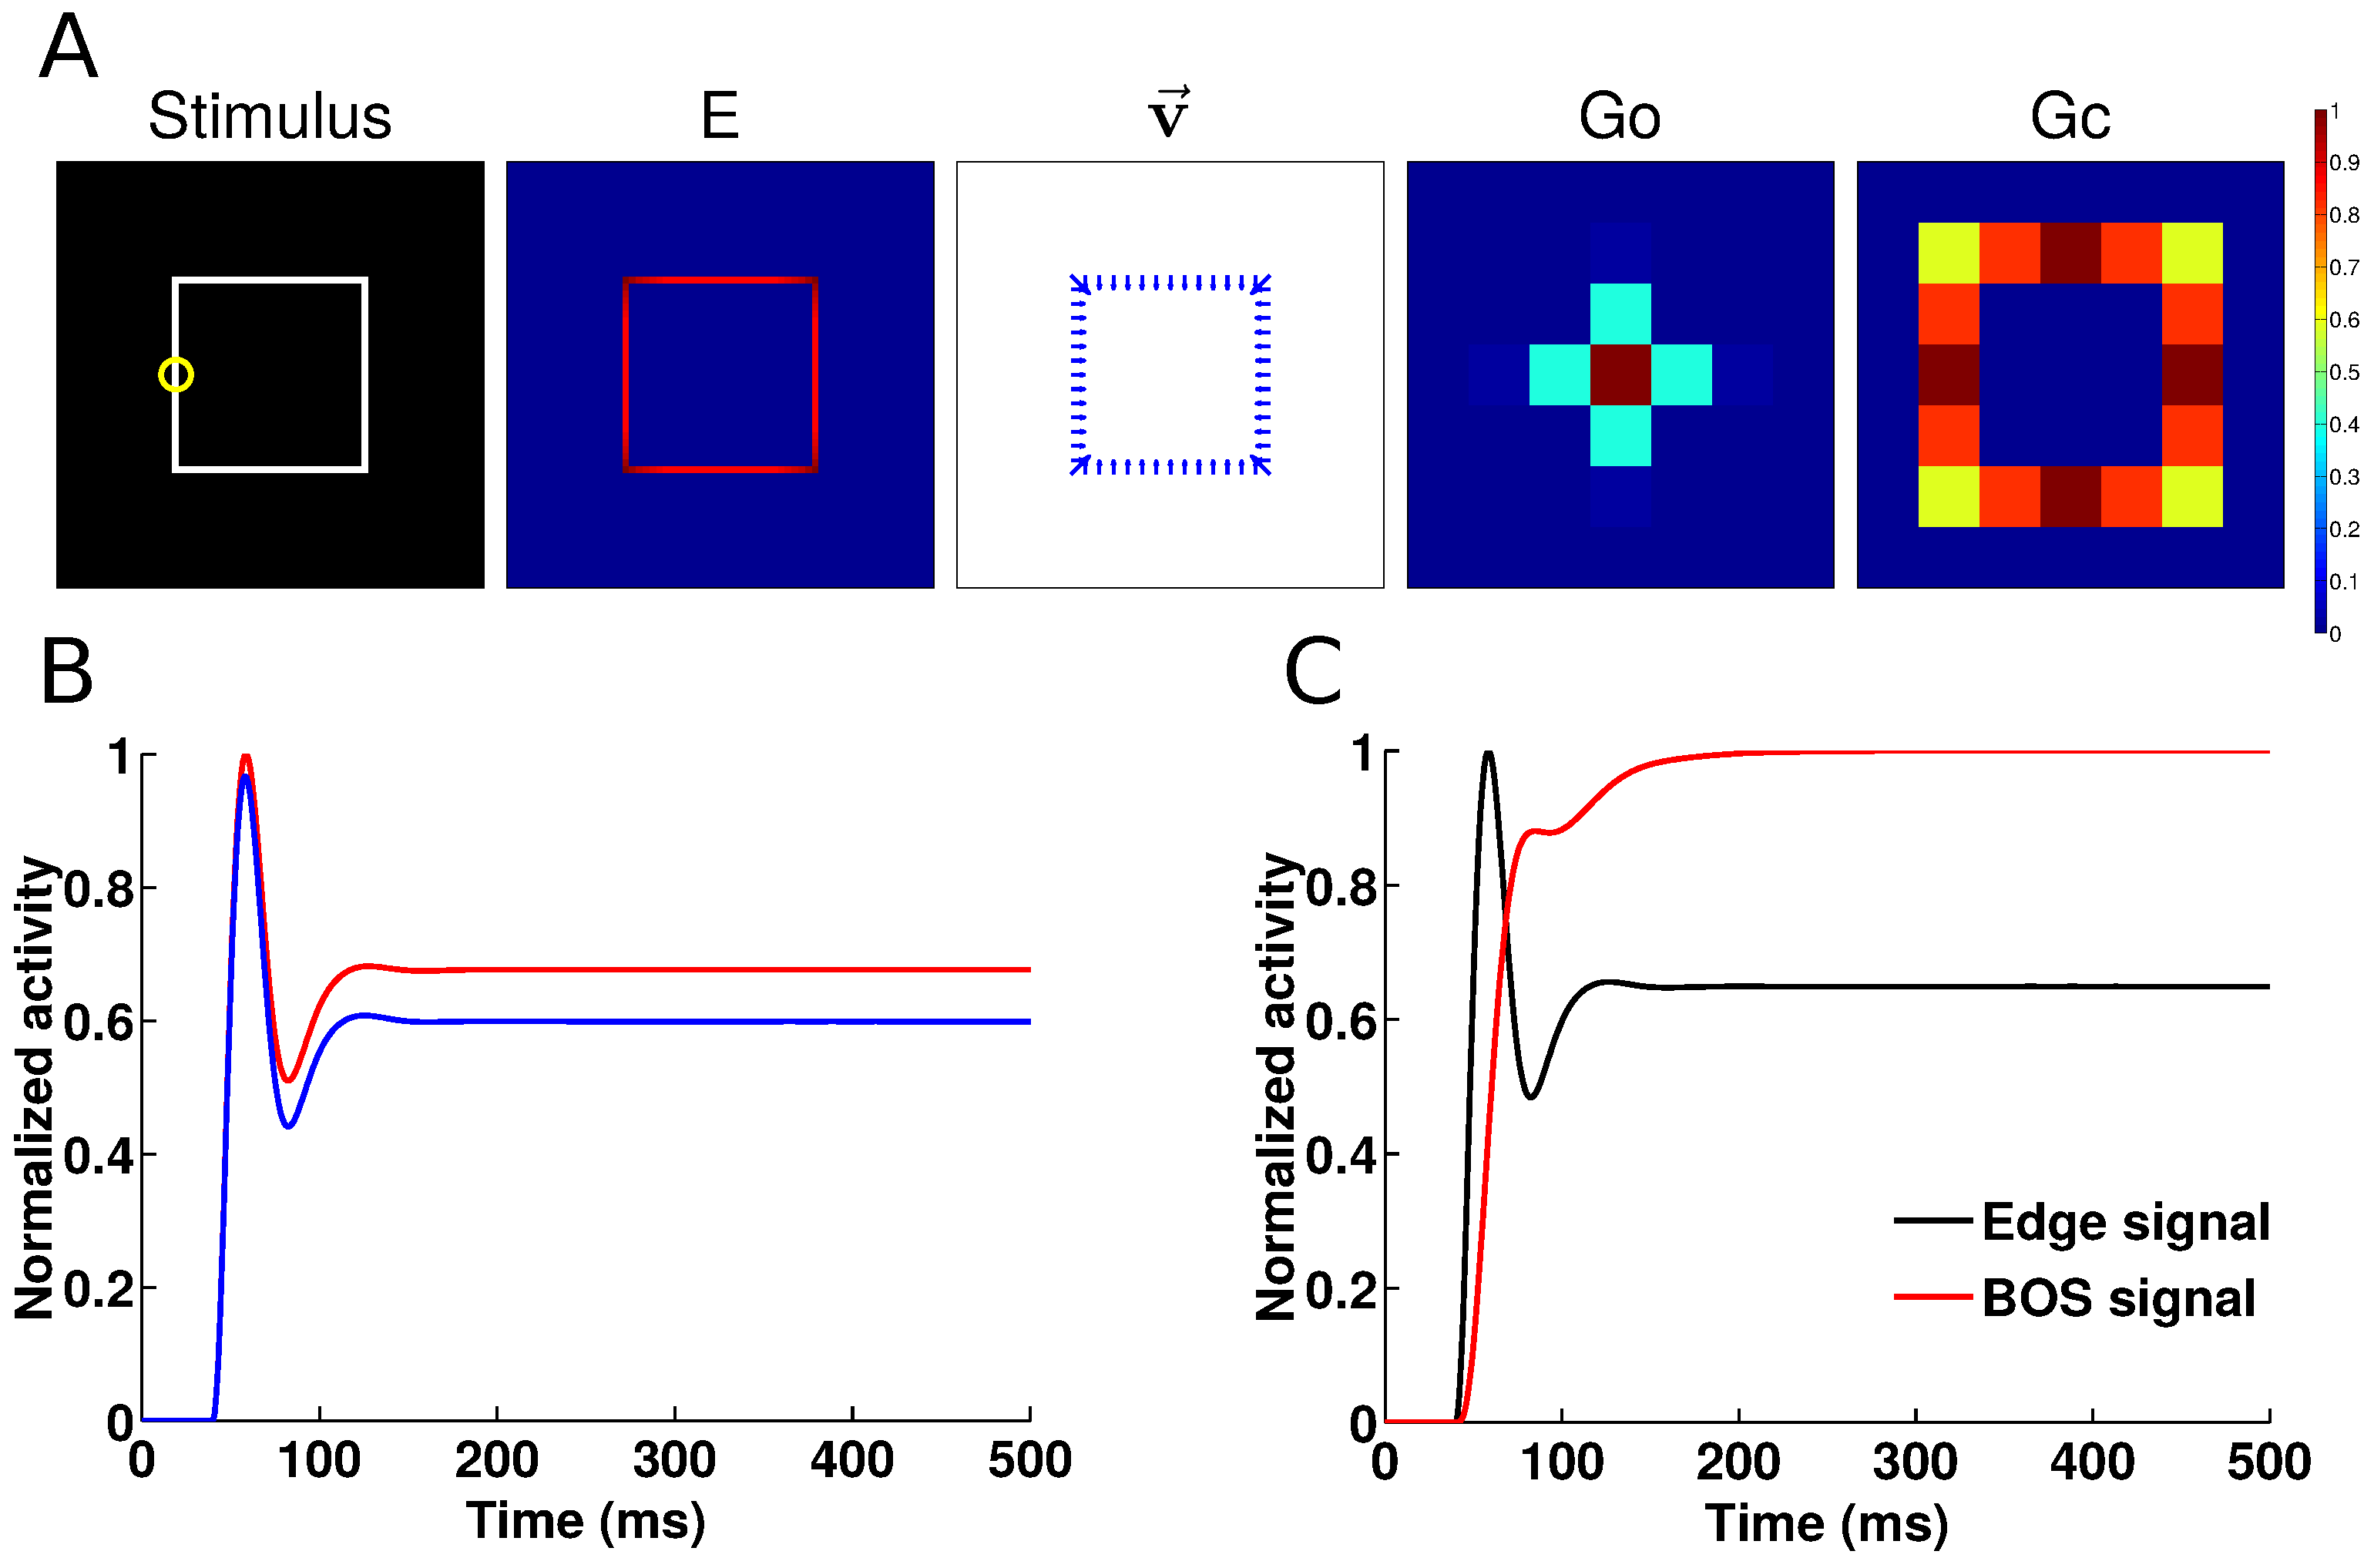
\includegraphics[width=\textwidth]{Contour/figs/Fig6.eps}
\makeatletter
\let\@currsize\normalsize
\caption[Figure-ground segregation with and without noise]{Figure-ground segregation of a square object with (bottom
row) and without (top row) noise. Shown are (left to right) the input
stimulus, the edge cell activity (E), the border ownership assignment along edges (shown as the vector modulation index $\vec{v}$, section~\ref{sec:vmi}), the object grouping neuron activity $(G_o)$
 and the contour grouping activity $(G_c)$.  Activities are normalized within each map, and warmer colors indicate higher activity (see color bar at right).}
\label{Fig:Square}
\end{figure}

\subsection{Border ownership assignment and highlighting figures in noise}
\label{sec:BOS}

We next apply our model to understanding border ownership assignment,
discussed in Section~\ref{sec:FGO}. We focus first on the standard
square figure frequently used in neurophysiological studies of this
function
\citep{Zhou_etal00,Qiu_etal07,Sugihara_etal11,Williford_vonderHeydt13,Williford_vonderHeydt14,Martin_vonderHeydt15}.
In Figure~\ref{Fig:Square}, we show the input stimulus, the edge cell
activity from area V1 of our model, the border ownership vector
modulation field from V2 (defined in Section~\ref{sec:vmi}), and the
object and contour grouping cell activity from V4.  The top row in the
figure shows that our model enhances V1 activity along the edges of
the square, correctly assigns border ownership towards the center of
the square in V2 neurons \citep[in agreement with][] {Zhou_etal00},
and highlights the center of the square and the edges of the square in
V4 neurons (object and contour grouping neurons, respectively).

We then extend this approach by adding strong stimulus noise which was
chosen as a large number of randomly oriented bars, similar to the
stimuli from the~\cite{Chen_etal14} study. Results are shown in
the bottom row of Figure~\ref{Fig:Square}. The edges of the
square, even when broken up into different bars, are still enhanced
while the background bars are suppressed, especially within the
square.  Border ownership is still assigned correctly along the edge
of the square, but the noise results in occasional nonzero border
ownership cell activity at other points in the image as well. Grouping
cell activity is still centered on the square, and contour grouping
neurons still highlight the edges of the squares, but there is also
noticeably increased noise.

\subsection{Interaction between border ownership assignment and attention} 
\label{sec:BOS-att}

Although border ownership selectivity emerges independently of
attention~\citep{Qiu_etal07}, attention may help to facilitate
figure-ground segregation in the presence of noise.  For the square
with noise, we found that attention increases the responses of neurons
along the edge of the figure (unpaired t-test, $p=\num{2.32e-59}$) and
suppresses those in the center (unpaired t-test,
$p=\num{3.42e-8}$). In addition, attention increases border ownership
modulation along the edge of the figure (unpaired t-test,
$p=\num{1.37e-143}$) and increases the activity of object grouping
neurons in the center of the figure (unpaired t-test,
$p=\num{1.53e-239}$). All effects were small but highly significant,
and were based on the differences in summed activity of neurons along
the edge or center of the figure over a total of 100 simulations.

These results demonstrate that the object and contour grouping neurons
are able to assist with early level segmentation of a square object in
noise.  Previous experimental studies have only tested squares without
noise, although the effect of figures defined by broken contours has
been investigated before~\citep{Zhang_vonderHeydt10}.  Our results predict
that border ownership assignment and grouping are robust even in the
presence of noise, and that attention may further aid this process.

\begin{figure}[t]
\centering
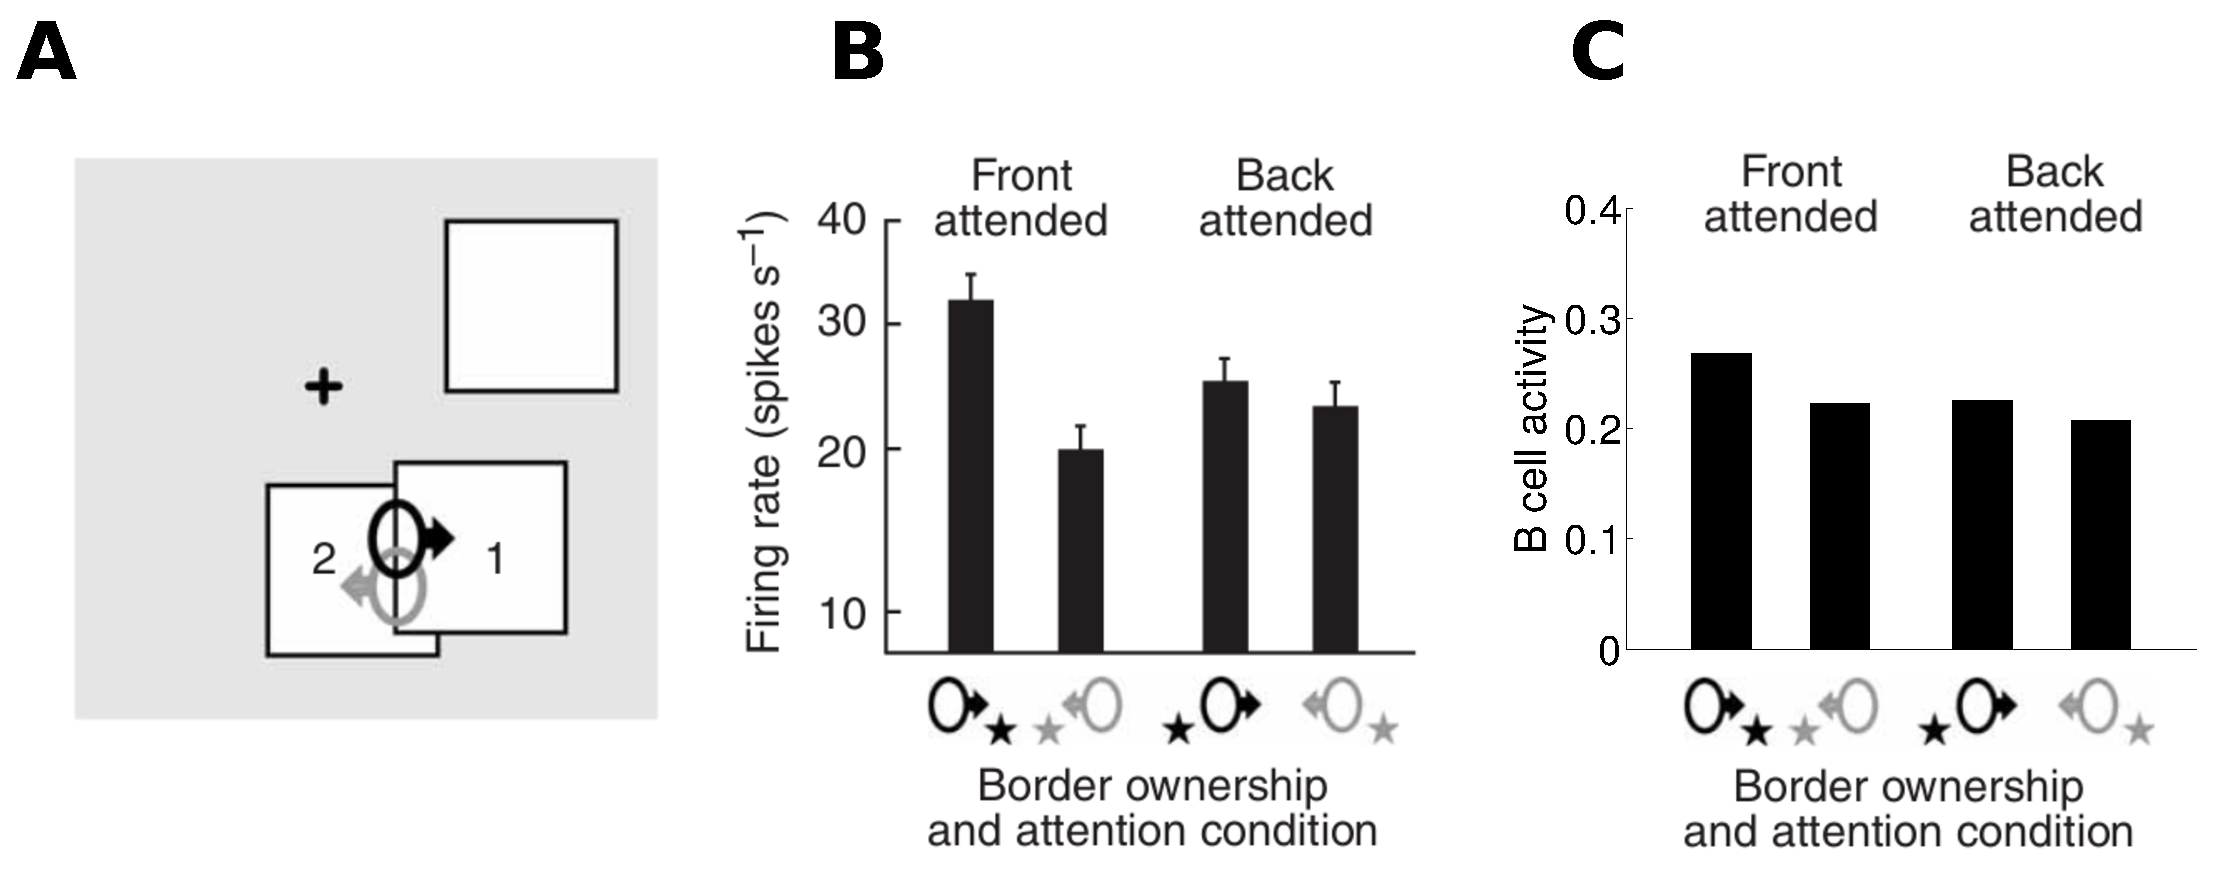
\includegraphics[width=\textwidth]{Contour/figs/Fig7.eps}
\makeatletter
\let\@currsize\normalsize
\caption[Comparison of model results to the Qiu et al. experiments]{Quantitative comparison of model performance to neurophysiological findings \citep{Qiu_etal07} for border-ownership coding of  overlapping figures. (A) The stimulus configurations used are shown, with neurons coding right border ownership (black) and left border ownership (gray) when attention was focused on either foreground square 1 (front attended) or on background square 2 (back attended). (B) The responses of border ownership selective cells recorded in V2 are shown:  bars indicate the average firing rate for each stimulus condition. (C) Model B cell responses to analogous stimulus conditions.
\comment{For both the model and the experiments, border-ownership modulation was strong when attention was on foreground but weak when attention was on background.}
Panels~A and~B are modified from Figure~3 of~\cite{Qiu_etal07}.}
\label{Fig:Overlap_Square_exp_model}
\end{figure}

\subsection{Border ownership assignment in the presence of multiple objects}
\label{sec:BOS_overlap}

Attention must operate in cluttered environments where multiple
objects may be present.~\cite{Qiu_etal07} studied border ownership
responses in area V2 when two overlapping squares were presented and
attention was directed either to the foreground or background square
(Figure~\ref{Fig:Overlap_Square_exp_model}A). Our model reproduces the
experimental finding that border-ownership modulation was strong when
attention was on the foreground figure but weak when attention was on
the background figure (compare
Figure~\ref{Fig:Overlap_Square_exp_model}B and
Figure~\ref{Fig:Overlap_Square_exp_model}C).
In our model, the approximate locations of the foreground and
background squares are represented by two peaks in the activity of
object grouping neurons (Figure~\ref{Fig:Overlap_Square}, fourth
column). Selectively attending to one object enhances the activity of
grouping neurons corresponding to the attended object while
simultaneously suppressing the activity of grouping neurons
representing the unattended object. Attentional modulation at the
grouping neuron level is then propagated back to border ownership
selective neurons along object boundaries via the feedback grouping
circuitry of our model.

\begin{figure}[t!]
\centering
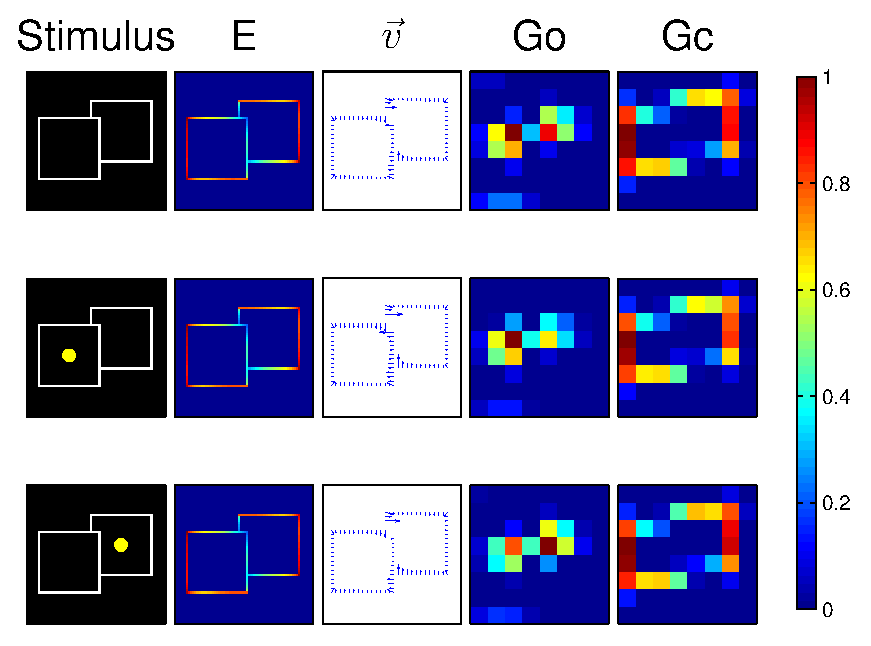
\includegraphics[width=0.75\textwidth]{Contour/figs/Fig8.eps}
\makeatletter
\let\@currsize\normalsize
\caption[Attention modulates border-ownership responses in the presence of multiple objects]{Attention in the presence of multiple objects. Shown are (left to right) the input stimulus, the edge cell activity (E), the border ownership assignment along edges (shown as the vector modulation index $\vec{v}$, section~\ref{sec:vmi}), the object grouping neuron activity (Go), and the contour grouping activity (Gc). Activities are normalized within each map, and warmer colors indicate higher activity (see color bar at right). The yellow dot indicates the locus of attention, which was applied at the level of grouping neurons. In the absence of attention (top row) or when attention is directed to the foreground square (middle row), the edge between the figures is correctly assigned to the foreground. If attention is directed toward the background square (bottom row), the border ownership signal of this edge is greatly reduced, consistent with experimental observations~\citep{Qiu_etal07}.}
\label{Fig:Overlap_Square}
\end{figure}

Even in the absence of attention, figure-ground segregation can be
observed in the border ownership assignment along the edges of the two
squares, as well as in the object and contour grouping cell activity
(Figure~\ref{Fig:Overlap_Square}, row 1).  Of particular interest is
the center edge separating the foreground and background squares. When
attention is directed to the foreground square, assignment of border
ownership along this edge is strengthened relative to the unattended
case (Figure~\ref{Fig:Overlap_Square}, row 2).  However, if attention
is directed toward the background square, border ownership modulation
of the edge between the two squares is greatly reduced
(Figure~\ref{Fig:Overlap_Square}, row 3).  These results are in
agreement with the physiological evidence~\citep{Qiu_etal07}, and
demonstrate that grouping mechanisms provide a means to attend to
objects in clutter.
Functionally, when attention is directed towards the occluded object,
suppression of the border ownership signal along the occluding edge is
useful because this edge is ``owned'' by the occluder and should not
be included in the representation of the attended object
\citep{Craft_etal07}.

\section{Discussion}
\label{sec:discussion}

\comment{In this study, we use computational models to elucidate the role of
attention and feedback in contour and object processing. Different
from many models that are tailor-made to reproduce one set of experimental
results, we demanded that our model explain data
from two different sets of experimental approaches, (1)~contour
integration and (2)~figure-ground segregation.  We hypothesize that
these two processes are fundamentally linked in terms of the larger
goal of image understanding.  Using the same set of model parameters,
we reproduced several experimental findings and generated non-trivial
predictions.}  

\subsection{Model predictions}

Our model predicts that attentional modulation is specific to the
attended contour or object, 
rather than being defined purely
spatially. This is possible because, in our model, attention modifies firing
rates of grouping cells, rather than of elementary feature-coding
cells. Attending to the contour increases
contour-response $d'$ in both V1 and V4, consistent with experimental
results showing increased contour-related responses after animals had
been trained to perform a contour detection task, compared to when
they performed a separate set of tasks in which the contour was
behaviorally irrelevant~\citep{Li_etal08a}. We note that
\cite{Li_etal08a} only studied neural responses in V1, while our model
makes predictions about attention-related changes to contour-response
$d'$ in both V1 and V4.
%bh Make this statement more general to encapsulate our results across V1, V2, and V4
We also find that attention modulates border ownership activity in V2 in an object-based manner. As a result, our model makes predictions about neural activity in visual areas
V1, V2, and V4 across different stimuli and tasks.
%

We predict that
the interaction of modulatory feedback from grouping cells with local
inhibition enhances the representation of the figure and suppresses
the representation of the background. 
Indeed, our model produces background suppression for
isolated contours as well as for figures embedded in noise.
We note that this prediction is different from what others have observed in
texture-defined figures \citep{Lamme95,Lee_etal98a}, where there is
generally response enhancement
of the center of the figure.
 This difference may be due to how the figure is defined,
by its contour in our experiment and by texture in
\cite{Lamme95,Lee_etal98a}. We also predict that attention, in
addition to enhancing the figure in an object-based manner, also helps
to suppress noise in the background. 

We also predict that removing feedback from V4 to lower visual areas
reduces neural responses in V1, while having a smaller effect in V4.
The activity of V4 neurons is also affected due to the recurrency of
the network model. 
This could be tested experimentally by the same contour
detection task used by~\cite{Chen_etal14}, and measuring the
contour-response $d'$ in V1 and V4 from reversible inactivation of
feedback connections. Although complete and selective deactivation of
V4 feedback to areas V1 and/or V2 is technically challenging, there
have been attempts to study the effect of this type of feedback either
through extra-striate lesions~\citep{Super_Lamme07} or reversible
inactivation~\citep{Jansen_etal12}.  Anesthesia presumably also
decreases top-down influences, and indeed reduces contour-related V1
responses \citep{Li_etal08a} and figure-ground segregation
\citep{Lamme_etal98}.

\subsection{Comparison to other models}

Many have argued that contour integration and figure-ground
segregation are largely local phenomena that rely on lateral
connections \citep{Grossberg94, Grossberg97, Li98, Zhaoping05,
  Piech_etal13}.  While some models include a role for top-down
influences \citep{Li98,Piech_etal13}, they do not offer a specific
mechanism by which higher visual areas representing object-level
information selectively feed back to lower visual areas containing
feature-level information about the object.  In contrast, our model is
explicit in that feedback connections from higher visual areas
modulate the responses of early feature-selective neurons involved in
the related processes of contour integration and figure-ground
segregation; as such it can be seen as more detailed implementation of
other, more conceptual models \citep{Piech_etal13,Poort_etal12}. One
limitation of these latter models is that they either represent local
processing within a single area or treat each intermediate area as a
relay to higher visual areas. As a result, they cannot reproduce the
neural responses in V4 for the contour integration experiments, nor
the findings in V2 for the figure-ground segregation experiments,
where most border ownership cells are found. Our model thus is a
member of a broad class of theoretical models that achieve image
understanding through bottom-up and top-down recurrent
processing~\citep{Ullman84,Hochstein_Ahissar02,Roelfsema_06,Epshtein_etal08}.

\subsection{Roles of V1 and V4 in visual processing}

While V1 neurons have small RFs that accurately code for orientation, V1 also shows strong
background inhibition off the contour. This property allows V1 neurons
to enhance contours and suppress noise in the image at a high spatial
resolution. V4 neurons, on the other hand, have large RFs that integrate
local feature information over large areas of visual space and provide
a coarse, proto-object representation of contours and objects.
Feedback from V4 can then be refined by the lateral connections present
within early visual areas, which aids in the enhancement of the figure
and its edges in the image.

Even when V1 neurons receive no feedback from V4, there is an
increase in contour-response $d'$ with contour length
(Figure~\ref{Fig:FB_att}). This contour facilitation is solely due to
the excitatory lateral connections present in V1, and is weaker
without feedback. As a result, feedback from V4 may not be necessary
for contour facilitation, but it interacts with local lateral
connections in a push-pull manner -- neurons along the contour are
enhanced, while elements on the background are suppressed. Not
surprisingly, removing this type of feedback has a larger effect on V1
neurons compared to V4 neurons, although the activity of V4 neurons is
also affected due to the recurrency of the network model.

\subsection{Contour and object grouping neurons}

Contour grouping neurons have direct experimental support through the
recent neurophysiological experiments published by~\cite{Chen_etal14}.
There is no clear neurophysiological evidence for object grouping
neurons yet, although previous studies have found neurons in V4 that
respond to contour segments of various
curvatures~\citep{Pasupathy_Connor02,Brincat_Connor04}. The receptive
fields of these neurons are similar to those proposed
 by~\cite{Craft_etal07}. Other types of grouping neurons may also exist,
including those that respond to gratings~\citep{Hegde_vanEssen07},
illusory surfaces~\citep{Cox_etal13}, or 3D
surfaces~\citep{He_Nakayama95,Hu_etal15a}.  We do not attempt to model
the whole array of grouping neurons that may exist, but only those
necessary for reproducing the neurophysiological experiments referred
to here.

In our model, orientation-independent attentional input to contour
grouping cells was used to enhance neural responses to a contour at a
given location.  We note that this form of attention is analogous to
the size- and location tolerant attentional selection process proposed
by~\cite{Mihalas_etal11b}. The local circuitry of their model was able
to sharpen a relatively broad and nonspecific attentional input to
match the size and location of a figure in the visual
scene. Similarly, the local circuitry of our model transforms the
orientation-independent attentional input such that it only enhances
the contour of the correct orientation. With this form of attention,
there is generalization over features for a given (approximate)
location.

Complementarily, feature-based attention acts broadly across the
visual scene and increases the responses of all components that share
similar feature attributes (\eg color, orientation, or direction of
movement) with the attended
component \citep{Motter94a,Treue_Trujillo99}.
Orientation-specific forms of attention
can enhance neural
responses in V1 and V4, but do not significantly alter
tuning curves or selectivity~\citep{McAdams_Maunsell99a}. 
Our model may be able to reproduce similar results by essentially changing the
form of the attentional input to be orientation-specific, \ie top-down
attention targets a \emph{single} population of contour grouping
neurons with the same orientation preference.
We expect that both
object-based and feature-based forms of attention exist and can be
flexibly used for different tasks.

\section{Conclusion}

Our model reproduces two different sets of experimental
results, while making testable predictions for future experiments. 
We only included one scale of grouping neurons for
simplicity, although 
multiple scales of grouping
neurons are needed to account for the diversity in the scale of
objects in the real world.
Our model also assigns distinct roles to the
different visual areas,  edge processing in V1, border ownership
assignment in V2, and grouping of contours and objects in V4. However,
the physiological properties of neurons in early visual areas have not
been fully characterized, and 
neurons in these different
areas may have 
additional ranges of selectivity
than the ones we assign them in our model. 
Finally, our model operates on artificial
images composed of simple shapes such as contours or square
figures. In order to truly understand grouping mechanisms in natural
vision, our model must also be able to operate on natural images as
input, where the number of potential objects and features are much
richer. We propose such a model in the next chapter.

%%% Local Variables:
%%% mode: latex
%%% TeX-master: "../root"
%%% End:
